\chapter{Desenvolvimento e Resultados}
\label{cap:desenvolvimento}

Este capítulo descreve cada um dos seis módulos do infográfico,
apresentando: (i)~o conceito teórico que o módulo materializa,
(ii)~as sub-abas que dividem o conteúdo, (iii)~as tabelas e dados
incorporados e (iv)~as simulações interativas implementadas em
JavaScript. Reproduções das telas são apresentadas como
Figuras~\ref{fig:mod1}--\ref{fig:mod6} (capturadas em
3 de junho de 2026, navegador Firefox).

\section{Arquitetura geral do infográfico}
\label{sec:arq-geral}

O artefato organiza-se segundo uma navegação lateral com sete itens:
seis módulos temáticos mais o índice de referências bibliográficas.
Cada módulo, por sua vez, divide-se em quatro sub-abas que isolam um
recorte conceitual --- decisão de design tomada na segunda iteração
para reduzir a densidade visual percebida na primeira versão.

A Listagem~\ref{lst:nav} mostra o esqueleto de navegação:

\begin{lstlisting}[language=HTML,label=lst:nav,caption=Esqueleto da navegação lateral]
<nav>
  <button onclick="showModule('mod1', this)">Desktop vs Servidor</button>
  <button onclick="showModule('mod2', this)">RAID Interativo</button>
  <button onclick="showModule('mod3', this)">Memória ECC</button>
  <button onclick="showModule('mod4', this)">Hierarquia & NUMA</button>
  <button onclick="showModule('mod5', this)">Virtualização</button>
  <button onclick="showModule('mod6', this)">Stack Completo</button>
  <button onclick="showModule('modRef', this)">Referências</button>
</nav>
\end{lstlisting}

Internamente, cada módulo é uma \texttt{section} com
\texttt{display:none} por padrão; a função \texttt{showModule()}
ativa apenas a seção solicitada (Listagem~\ref{lst:showmodule}).

\begin{lstlisting}[language=JavaScript,label=lst:showmodule,caption=Função de navegação principal]
function showModule(modId, element) {
    document.querySelectorAll('.module').forEach(m =>
        m.classList.remove('active'));
    document.querySelectorAll('.nav-btn').forEach(b =>
        b.classList.remove('active'));
    document.getElementById(modId).classList.add('active');
    if (element) element.classList.add('active');
    window.scrollTo({ top: 0, behavior: 'smooth' });
}
\end{lstlisting}

\section{Módulo 1 --- Desktop \textit{vs.}\ Servidor}
\label{sec:mod1}

\begin{figure}[h!]
\centering
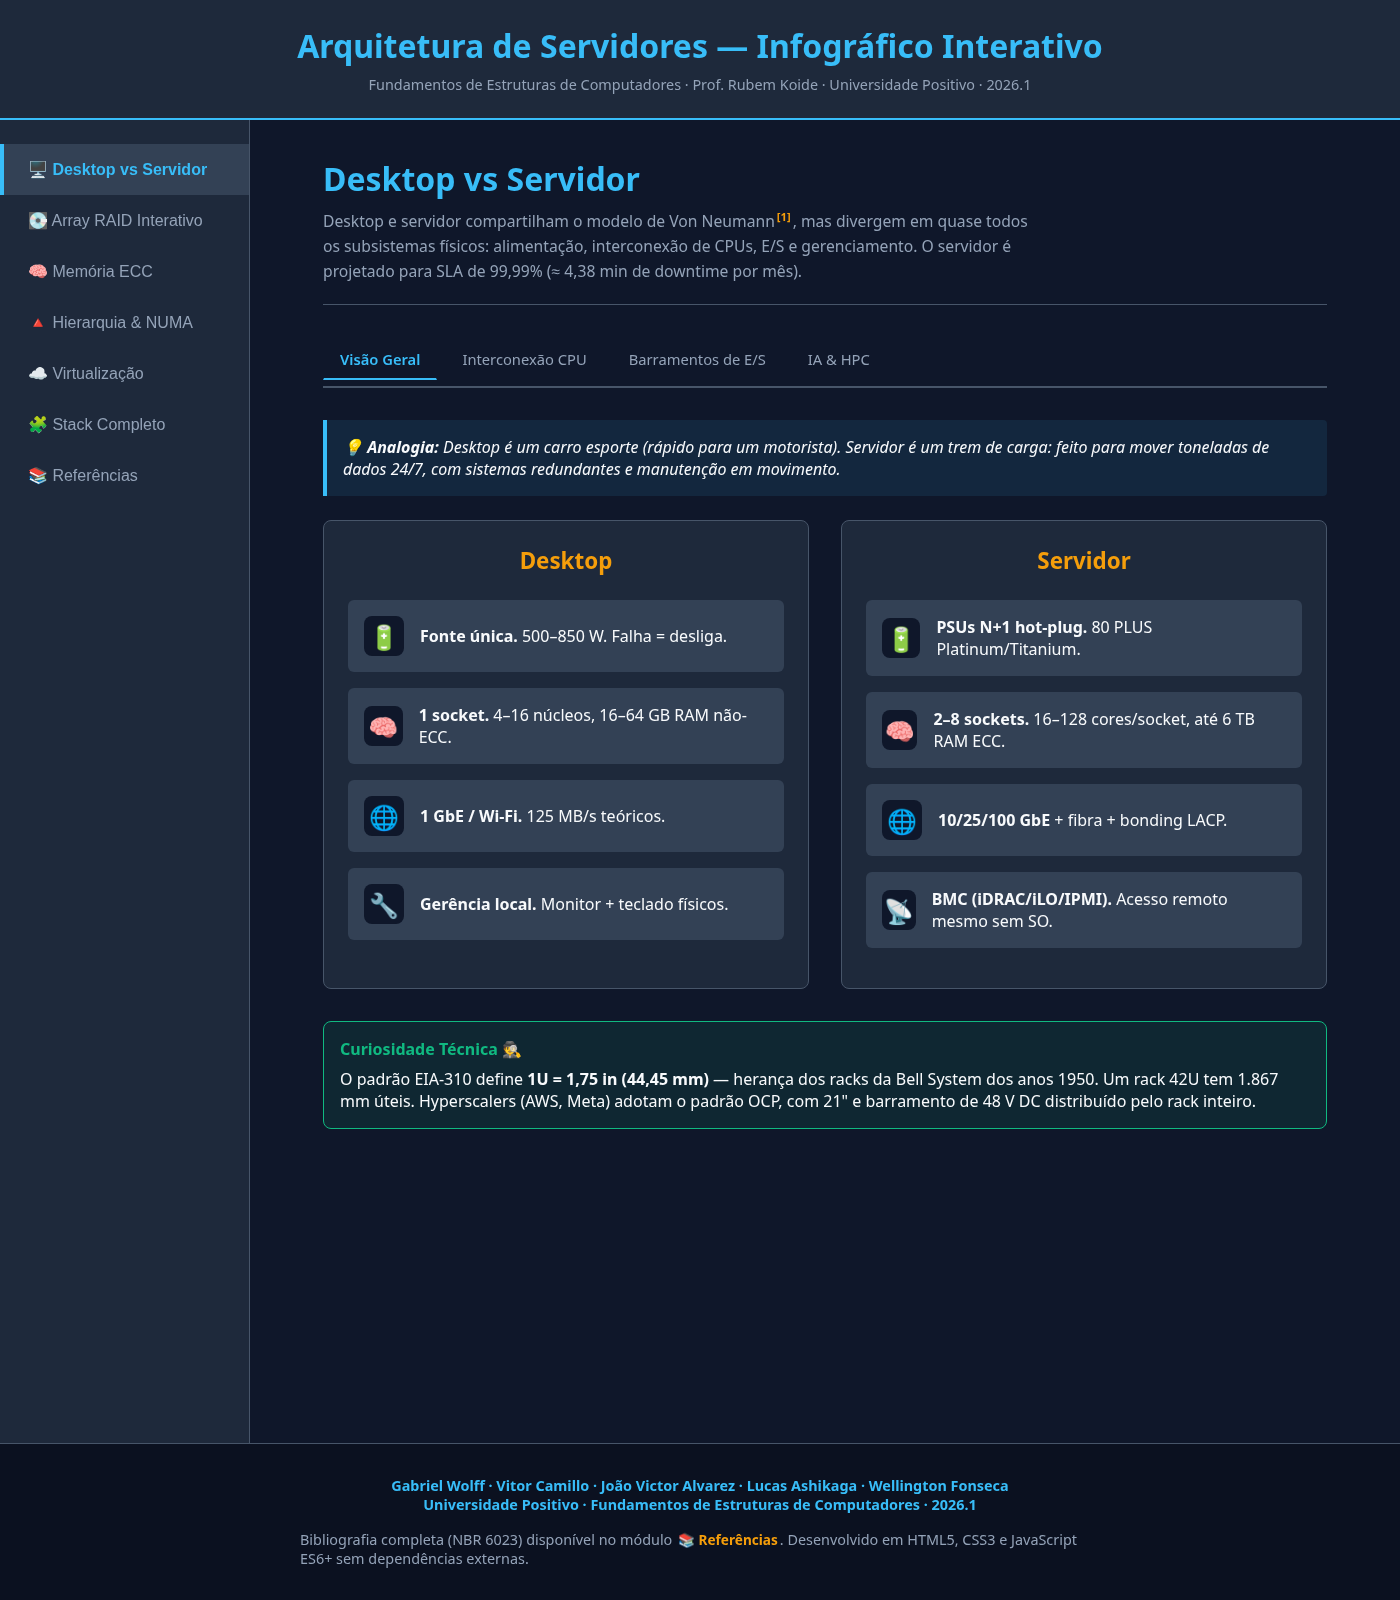
\includegraphics[width=0.95\textwidth]{figuras/mod1.png}
\caption{Módulo 1 --- Comparativo Desktop \textit{vs.}\ Servidor.}
\label{fig:mod1}
\end{figure}

O módulo apresenta quatro sub-abas:

\begin{description}
    \item[Visão Geral] grade comparativa lado-a-lado com 4 itens
          em cada coluna (alimentação, sockets, rede, gerência),
          mais analogia didática e curiosidade técnica sobre o
          padrão EIA-310.
    \item[Interconexão CPU] diagrama \emph{dual-socket} com link
          \textsc{upi} explícito (41,6\,\textsc{gb/s},
          \textasciitilde 100\,\textsc{ns}) e tabela comparativa de
          \textsc{fsb}, \textsc{qpi}, \textsc{upi}, Infinity Fabric
          e \textsc{nv}Link.
    \item[Barramentos de E/S] tabela quantitativa de
          \textsc{pci}e 3.0/4.0/5.0, \textsc{nvme}, \textsc{sata},
          1/10/100\,\textsc{gbe} e \textsc{InfiniBand}, com
          \textit{throughput} em \textsc{gb/s}.
    \item[IA \& HPC] cards com servidores de inteligência
          artificial: \textsc{nvidia} Grace Hopper GH200, AMD
          Instinct MI300X, Google TPU v5p e os supercomputadores
          \emph{El Capitan} (LLNL, nº\,1 do TOP500 desde nov/2024 com
          1,809\,\textsc{efl}\textsc{op/s}) e \emph{Frontier} (Oak
          Ridge, nº\,2 com 1,353\,\textsc{efl}\textsc{op/s}).
\end{description}

\subsection{Tabela comparativa de interconexões}

A Tabela~\ref{tab:mod1-interconexao} é a peça central da aba
``Interconexão CPU''. Os números provêm do \emph{white paper} da
Intel~\cite{intel2009qpi} e do material das aulas~\cite{koide2026}.

\begin{table}[h!]
\centering
\caption{Tecnologias de interconexão multi-socket}
\label{tab:mod1-interconexao}
\begin{tabular}{llrl}
\toprule
\textbf{Tecnologia} & \textbf{Fabricante} & \textbf{Banda} &
\textbf{Coerência} \\
\midrule
FSB             & Intel até 2008   & 10,6 GB/s  & Snooping \\
QPI             & Intel 2008--2017 & 25,6 GB/s  & MESIF (5 camadas) \\
UPI             & Intel Skylake+   & 41,6 GB/s  & MESIF + diretório \\
Infinity Fabric & AMD              & 204 GB/s   & MOESI \\
NVLink 4.0      & NVIDIA           & 900 GB/s   & GPU coherency \\
\bottomrule
\end{tabular}
\end{table}

\section{Módulo 2 --- RAID Interativo}
\label{sec:mod2}

\begin{figure}[h!]
\centering
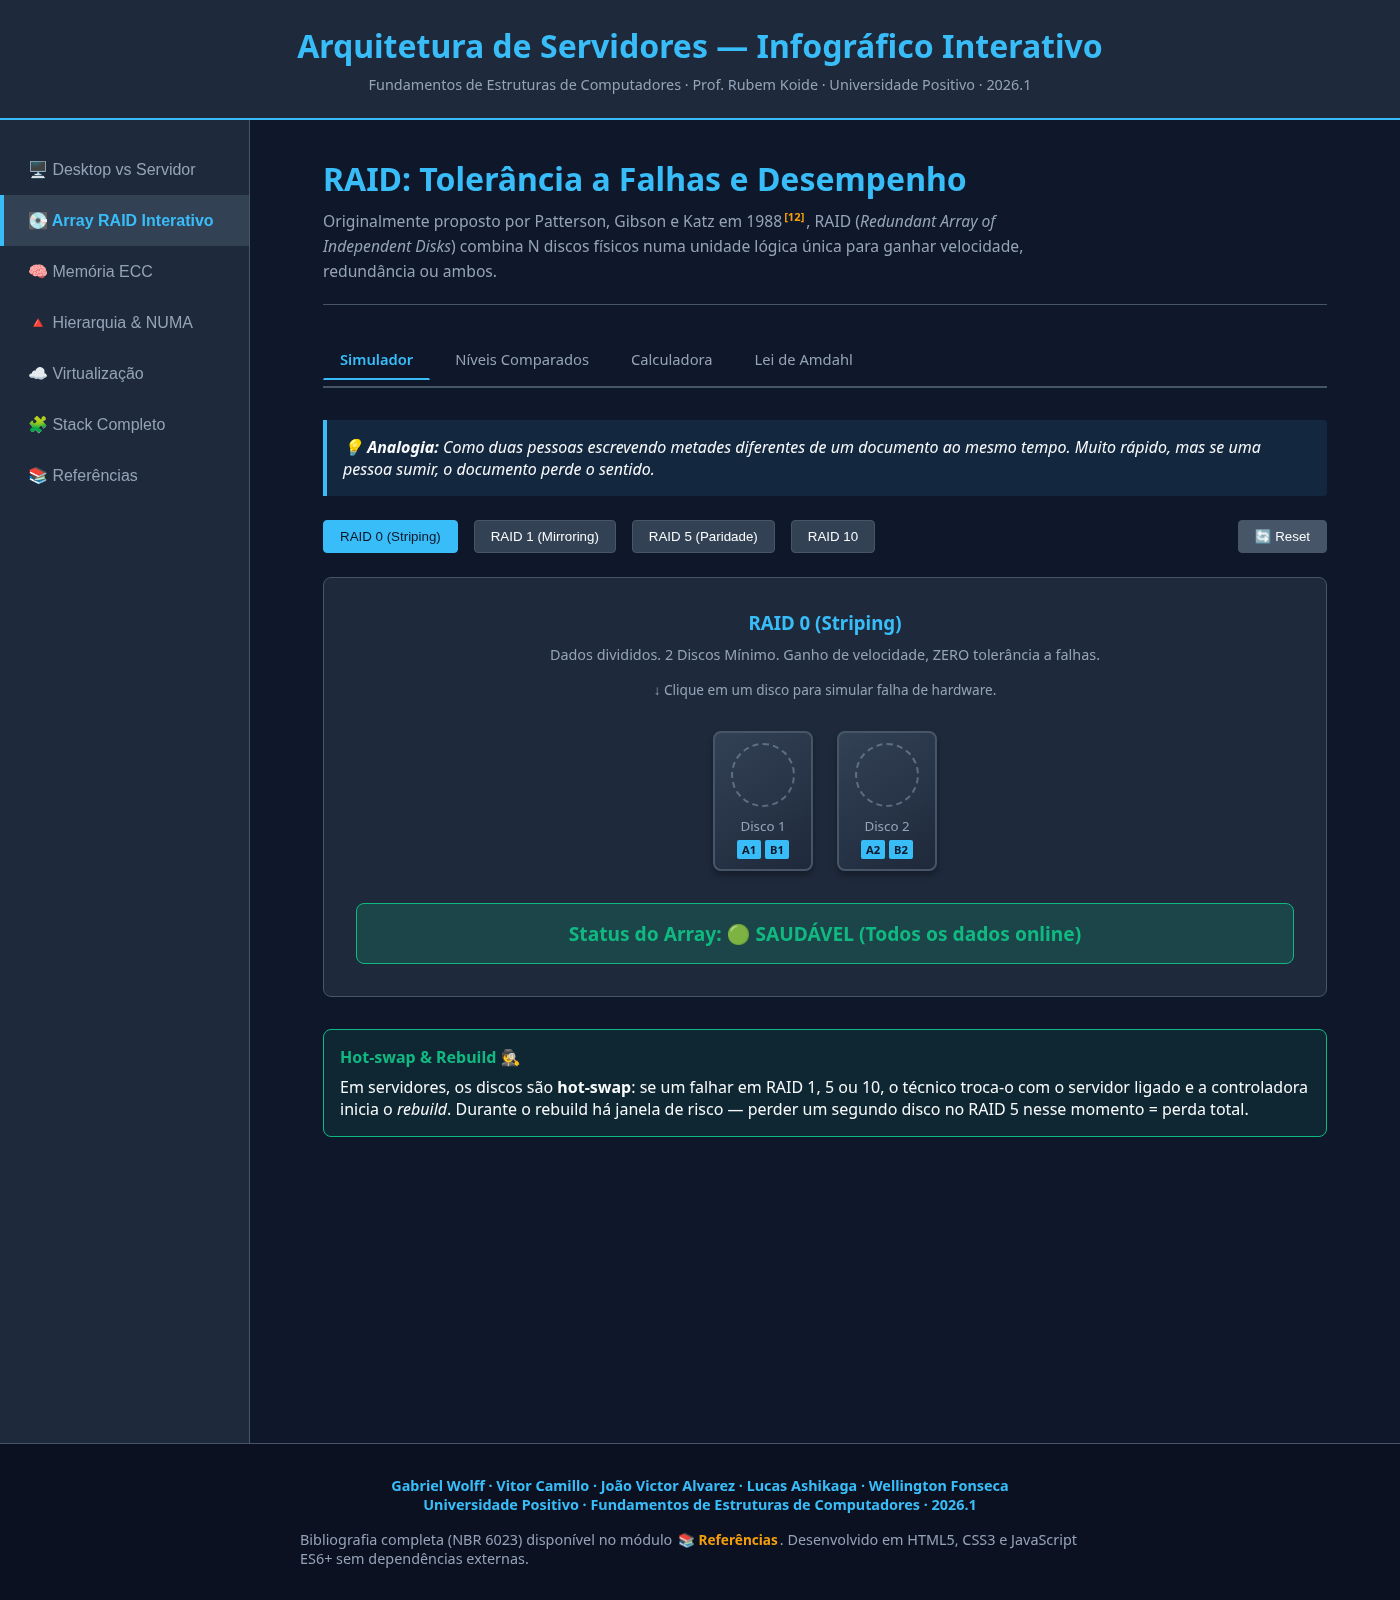
\includegraphics[width=0.95\textwidth]{figuras/mod2.png}
\caption{Módulo 2 --- RAID com simulador de falha.}
\label{fig:mod2}
\end{figure}

Distribuído em quatro sub-abas:

\begin{description}
    \item[Simulador] reproduz a versão original do módulo --- o
          aluno seleciona o nível \textsc{raid} (0, 1, 5 ou 10), o
          sistema desenha os discos e calcula em tempo real o
          impacto de cliques sucessivos (falhas) sobre o
          \emph{status} do \emph{array}.
    \item[Níveis Comparados] tabela com seis níveis (0, 1, 5, 6, 10,
          50) detalhando capacidade útil, tolerância e penalidade de
          escrita, mais a fórmula explícita de paridade
          $P = A \oplus B \oplus C$.
    \item[Calculadora] formulário onde o usuário escolhe nível,
          número de discos, capacidade individual e \textsc{iops} por
          disco; o sistema computa capacidade útil, eficiência de
          espaço, discos toleráveis e \textsc{iops} de leitura/escrita
          considerando a penalidade do nível selecionado.
    \item[Lei de Amdahl] aplicação numérica do
          Capítulo~\ref{cap:referencial}, com simulador interativo
          (\emph{slider} de fração paralelizável $P$ e número de
          discos $N$) que recalcula o \emph{speedup} efetivo e o
          teto teórico em tempo real.
\end{description}

\subsection{Lógica do simulador de falhas}

O estado do \emph{array} é mantido num vetor JavaScript
\texttt{raidState}; cada elemento descreve o ID do disco e se ele
está em falha. A função \texttt{updateRaidStatus()} contém o
\texttt{switch} que codifica o comportamento esperado de cada nível
sob diferentes contagens de falhas (Listagem~\ref{lst:raidstatus}).

\begin{lstlisting}[language=JavaScript,label=lst:raidstatus,caption=Trecho da lógica de status do RAID]
switch(currentRaid) {
    case 0:
        statusClass = 'status-fail';
        statusStr   = 'PERDA TOTAL! RAID 0 não tolera falhas.';
        break;
    case 1:
        if (failedCount === 1) { statusClass = 'status-warn';
            statusStr = 'DEGRADADO! Operando só pelo espelho.'; }
        else { statusClass = 'status-fail';
            statusStr = 'FALHA CRITICA! Ambos espelhos perdidos.'; }
        break;
    case 5:
        if (failedCount === 1) { statusClass = 'status-warn';
            statusStr = 'DEGRADADO! Recalculando paridade.'; }
        else { statusClass = 'status-fail';
            statusStr = 'RAID 5 só tolera 1 falha.'; }
        break;
    /* ... RAID 10 omitido por brevidade ... */
}
\end{lstlisting}

\subsection{Calculadora de IOPS}

A fórmula adotada para a penalidade de escrita segue a literatura
padrão de armazenamento empresarial:

\begin{equation}
\mathrm{IOPS}_{\text{escrita}} = \frac{N \cdot \mathrm{IOPS}_{\text{disco}}}{\text{penalty}}
\quad \text{com penalty} \in \{1, 2, 4, 6, 2\}
\end{equation}

para os níveis 0, 1, 5, 6, 10 respectivamente. Isso reproduz o
conhecido ``RAID~5 \emph{write penalty}'' de fator 4.

\section{Módulo 3 --- Memória ECC e Hamming \textsc{secded}}
\label{sec:mod3}

\begin{figure}[h!]
\centering
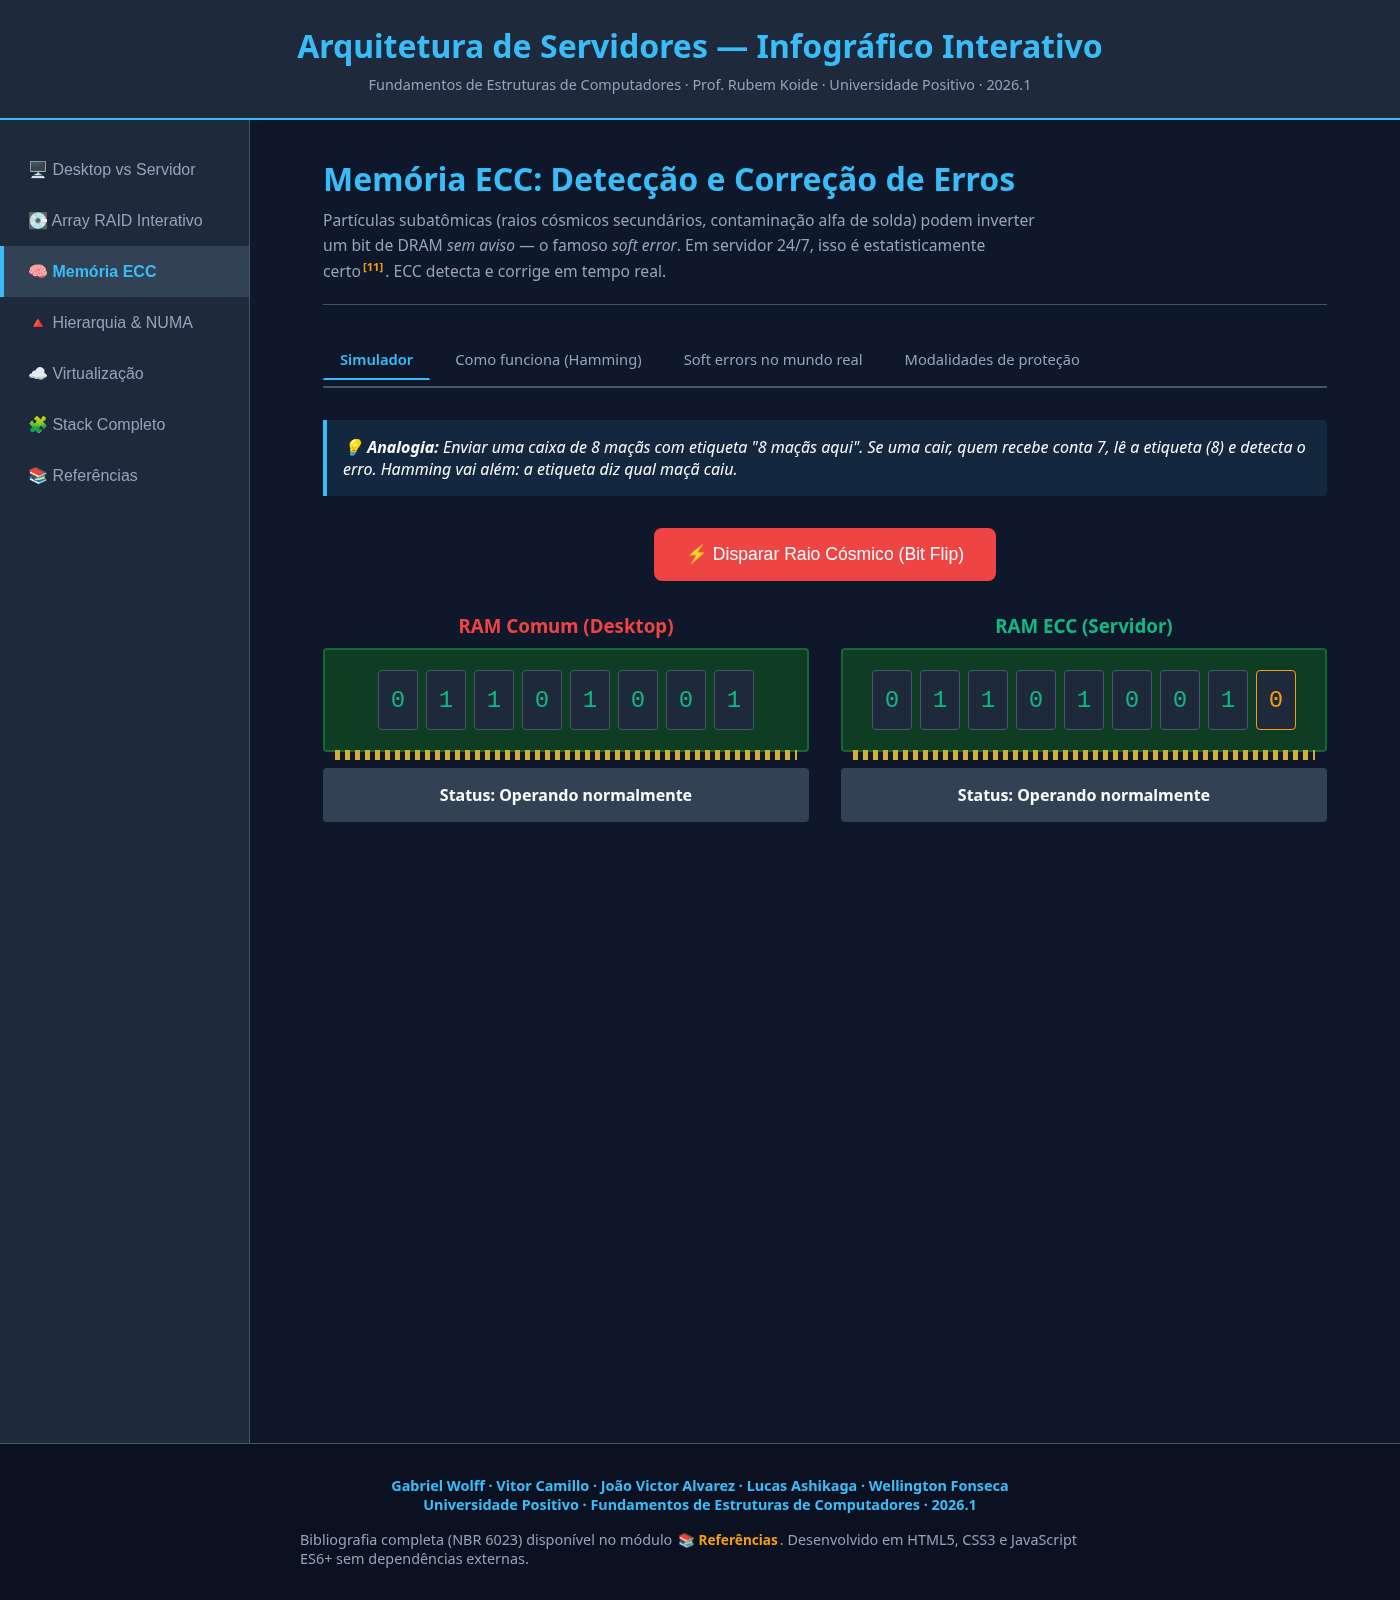
\includegraphics[width=0.95\textwidth]{figuras/mod3.png}
\caption{Módulo 3 --- Memória ECC: simulador de bit flip.}
\label{fig:mod3}
\end{figure}

Quatro sub-abas:

\begin{description}
    \item[Simulador] herda a animação original de raio cósmico,
          comparando lado-a-lado RAM comum e RAM \textsc{ecc}.
    \item[Como funciona (Hamming)] mostra os 12 bits da palavra
          Hamming(12,8) com correção de erro único (SEC): quatro
          paridades $P_1, P_2, P_4, P_8$ nas posições $2^k$, oito
          bits de dado, e a extensão para (13,8) (\textsc{secded})
          via bit de paridade global.
    \item[Soft errors no mundo real] expõe os números do estudo de
          Schroeder \textit{et al.}~\cite{schroeder2009} ---
          25\,000 a 70\,000 \textsc{fit} por \textsc{mb}it,
          mais de 8\,\% dos \textsc{dimm}s afetados por ano --- e
          cita o caso da eleição federal belga em Schaerbeek
          (2003), em que a candidata Maria Vindevoghel recebeu
          4\,096 votos extras por inversão de um único bit na
          posição 13 do contador, atribuída a um \emph{single-event
          upset} (hipótese provável, nunca comprovada definitivamente).
    \item[Modalidades de proteção] tabela comparando paridade
          simples, \textsc{secded}, Chipkill/\textsc{sddc} e
          \textsc{ddr5} \emph{on-die} \textsc{ecc}.
\end{description}

\subsection{Cálculo do síndrome}

Com 4 bits de paridade, a representação binária do \emph{síndrome}
recalculado na leitura tem 16 valores possíveis; 0 indica ausência
de erro, e os demais indicam exatamente a posição do bit
corrompido. Por exemplo: paridades $(s_3, s_2, s_1, s_0) = (0,1,0,1)$
$\Rightarrow$ posição decimal 5 $\Rightarrow$ corrupção em $D_2$
(o segundo bit de dado, na posição 5 do layout Hamming).

\section{Módulo 4 --- Hierarquia, Cache e NUMA}
\label{sec:mod4}

\begin{figure}[h!]
\centering
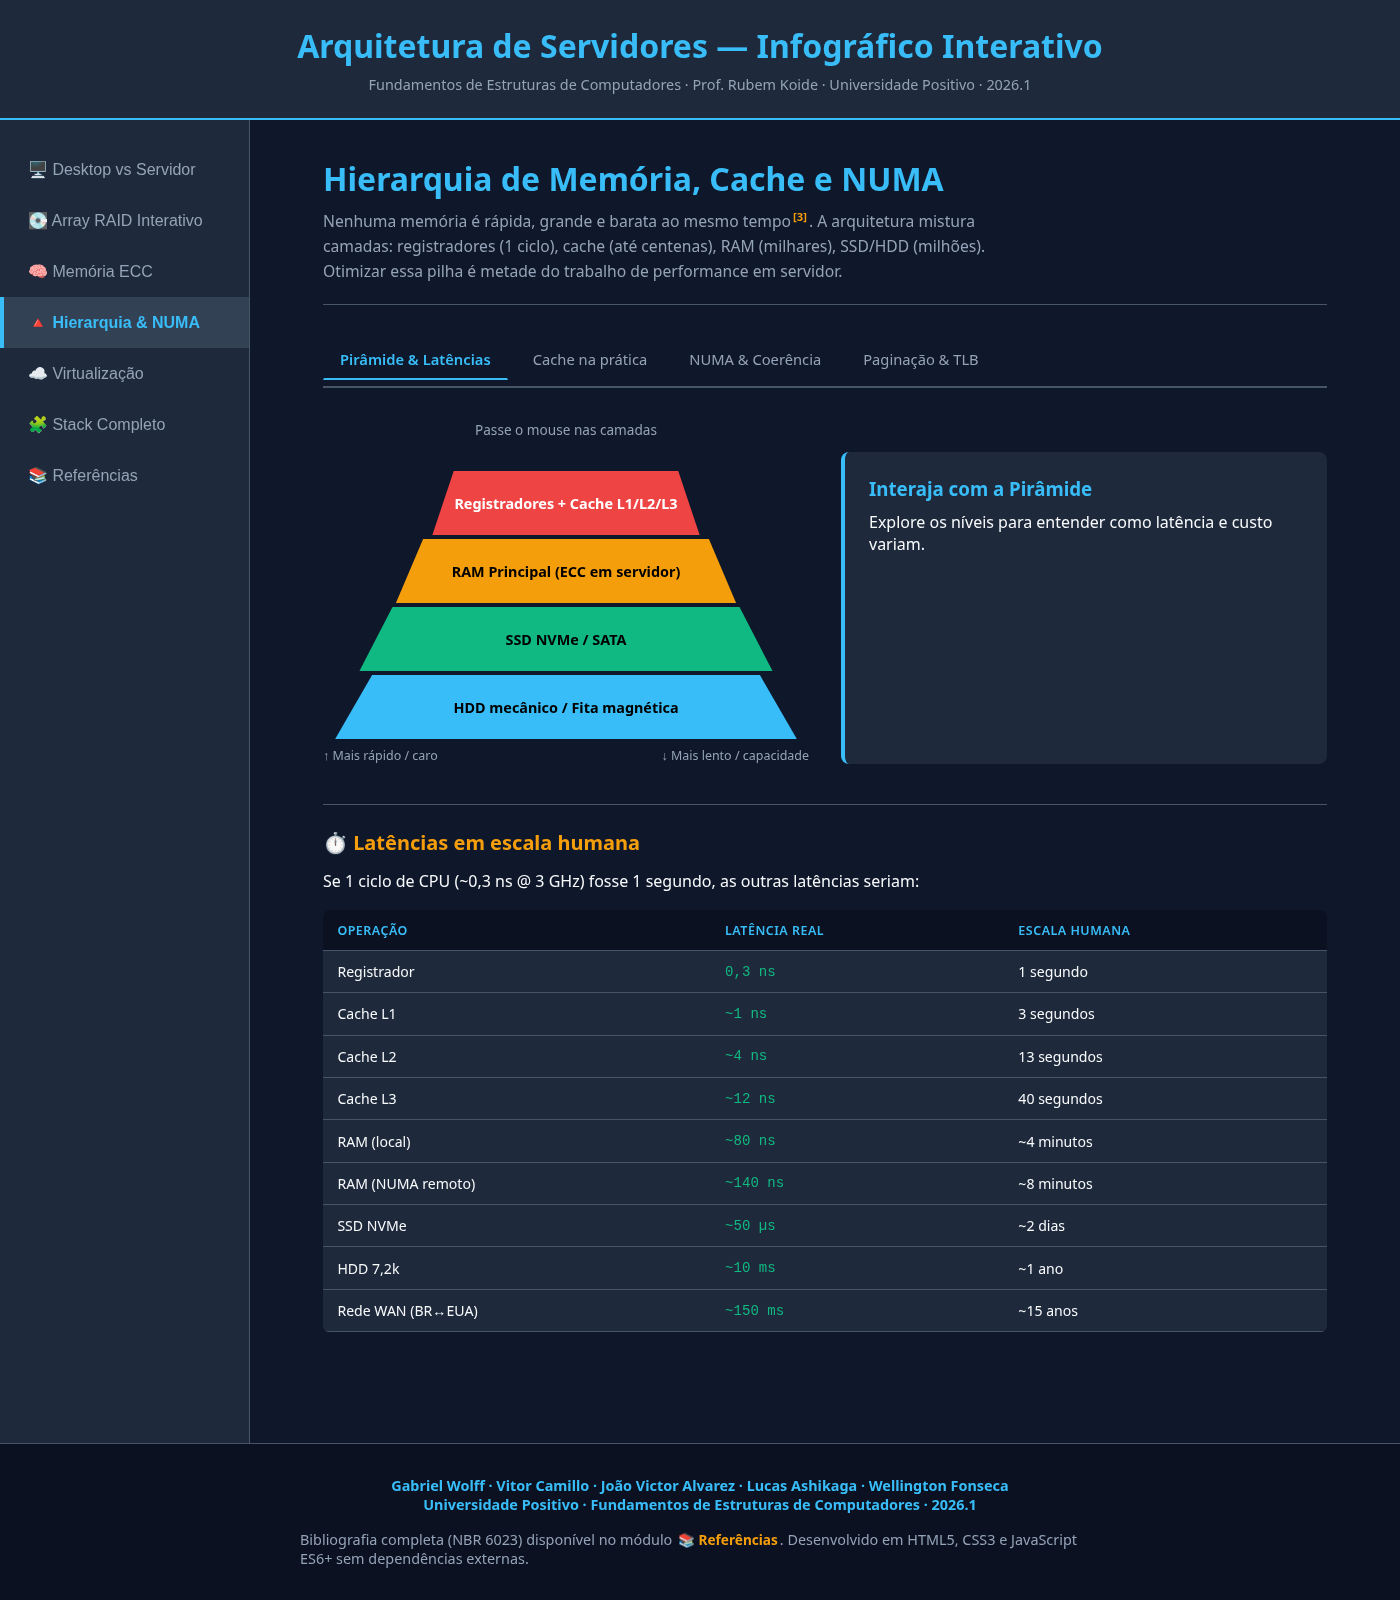
\includegraphics[width=0.95\textwidth]{figuras/mod4.png}
\caption{Módulo 4 --- Pirâmide de memória com latências em escala humana.}
\label{fig:mod4}
\end{figure}

Quatro sub-abas:

\begin{description}
    \item[Pirâmide \& Latências] versão original da pirâmide
          interativa com hover, complementada por uma tabela que
          escalona as latências para a referência humana (se 1
          ciclo de CPU equivalesse a 1 segundo, um acesso à RAM
          remota NUMA equivaleria a 8 minutos).
    \item[Cache na prática] tabela com a hierarquia real de um Intel
          Core i7-5960X (Tabela~\ref{tab:cache-i7}) e simulador de
          \emph{cache hit/miss} animado.
    \item[NUMA \& Coerência] diagrama \emph{dual-socket} com
          latência local (80\,\textsc{ns}) versus remota
          (140\,\textsc{ns}), e tabela explicando os 4 estados do
          protocolo \textsc{mesi}.
    \item[Paginação \& TLB] páginas de 4\,\textsc{kb} \emph{vs.}
          \textit{huge pages} de 2\,\textsc{mb}, \textit{page walk}
          em 4 níveis no x86-64, fórmula
          $t_{\text{acesso}} = t_{\text{tlb}} + (\text{taxa\_miss} \cdot t_{\text{pagewalk}})$.
\end{description}

\begin{table}[h!]
\centering
\caption{Cache do Intel Core i7-5960X (8 cores, Haswell-E)}
\label{tab:cache-i7}
\begin{tabular}{lrlrl}
\toprule
\textbf{Nível} & \textbf{Tamanho} & \textbf{Assoc.} &
\textbf{Latência} & \textbf{Escopo} \\
\midrule
L1d   & 32 KB  & 8-way  & 4 ciclos  & Por core \\
L1i   & 32 KB  & 8-way  & 4 ciclos  & Por core \\
L2    & 256 KB & 8-way  & 12 ciclos & Por core \\
L3    & 20 MB  & 20-way & 38 ciclos & 8 cores \\
\bottomrule
\end{tabular}
\end{table}

\subsection{Simulador de acesso à cache}

Implementa probabilidades empíricas típicas: 92\,\% de \textit{hit}
em L1, 6\,\% em L2, 1,5\,\% em L3 e 0,5\,\% \textit{miss} até a RAM.
A cada clique no botão ``Simular acesso'', a função
\texttt{simulateCacheAccess()} sorteia o resultado e anima a
travessia da pirâmide marcando \emph{miss} em cinza e \emph{hit} em
verde, exibindo o custo em ciclos do nível atingido.

\section{Módulo 5 --- Virtualização}
\label{sec:mod5}

\begin{figure}[h!]
\centering
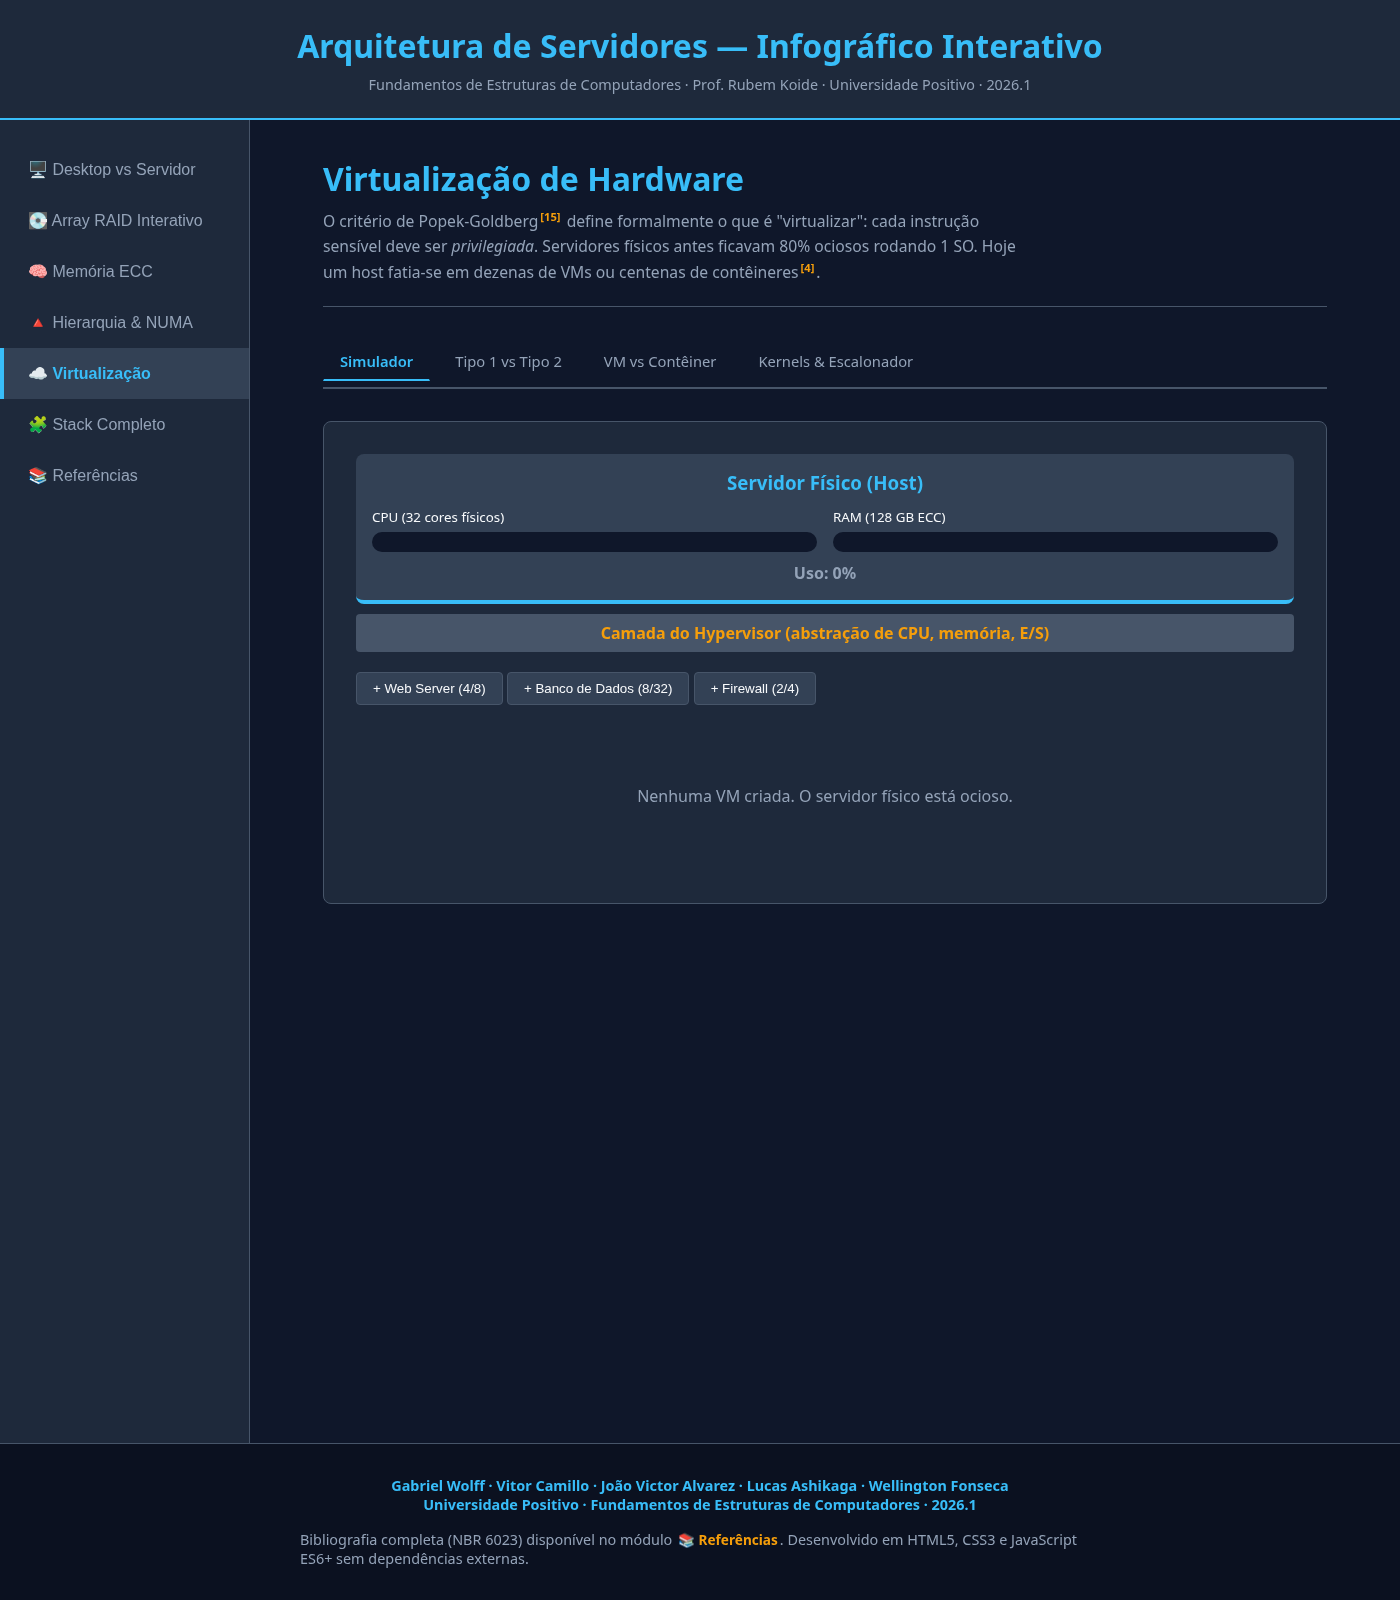
\includegraphics[width=0.95\textwidth]{figuras/mod5.png}
\caption{Módulo 5 --- Alocador de máquinas virtuais sobre o \emph{host} físico.}
\label{fig:mod5}
\end{figure}

Quatro sub-abas:

\begin{description}
    \item[Simulador] o alocador de VMs original, que limita a soma
          de v\textsc{cpu}s e RAM ao máximo físico (32 cores /
          128\,\textsc{gb}) e visualmente preenche barras de
          recurso, vermelha se acima de 80\,\%.
    \item[Tipo 1 \textit{vs.}\ Tipo 2] tabela taxonômica + diagrama
          dos anéis de proteção x86, incluindo o
          \textsc{vmx} \emph{root} (Ring~$-1$) introduzido por
          \textsc{vt-x}/AMD-V, e curiosidade sobre \textsc{wsl}~2
          como caso de virtualização leve.
    \item[VM \textit{vs.}\ Contêiner] tabela comparando granularidade,
          \emph{boot time}, \textit{footprint} e densidade, mais um
          trecho de código Linux mostrando criação manual de
          contêiner com \texttt{unshare} + \texttt{cgroups}.
    \item[Kernels \& Escalonador] comparação Windows NT (híbrido)
          \emph{vs.}\ Linux (monolítico modular), com diagrama da
          árvore rubro-negra usada pelo \textsc{cfs}.
\end{description}

\section{Módulo 6 --- \emph{Stack} Completo}
\label{sec:mod6}

\begin{figure}[h!]
\centering
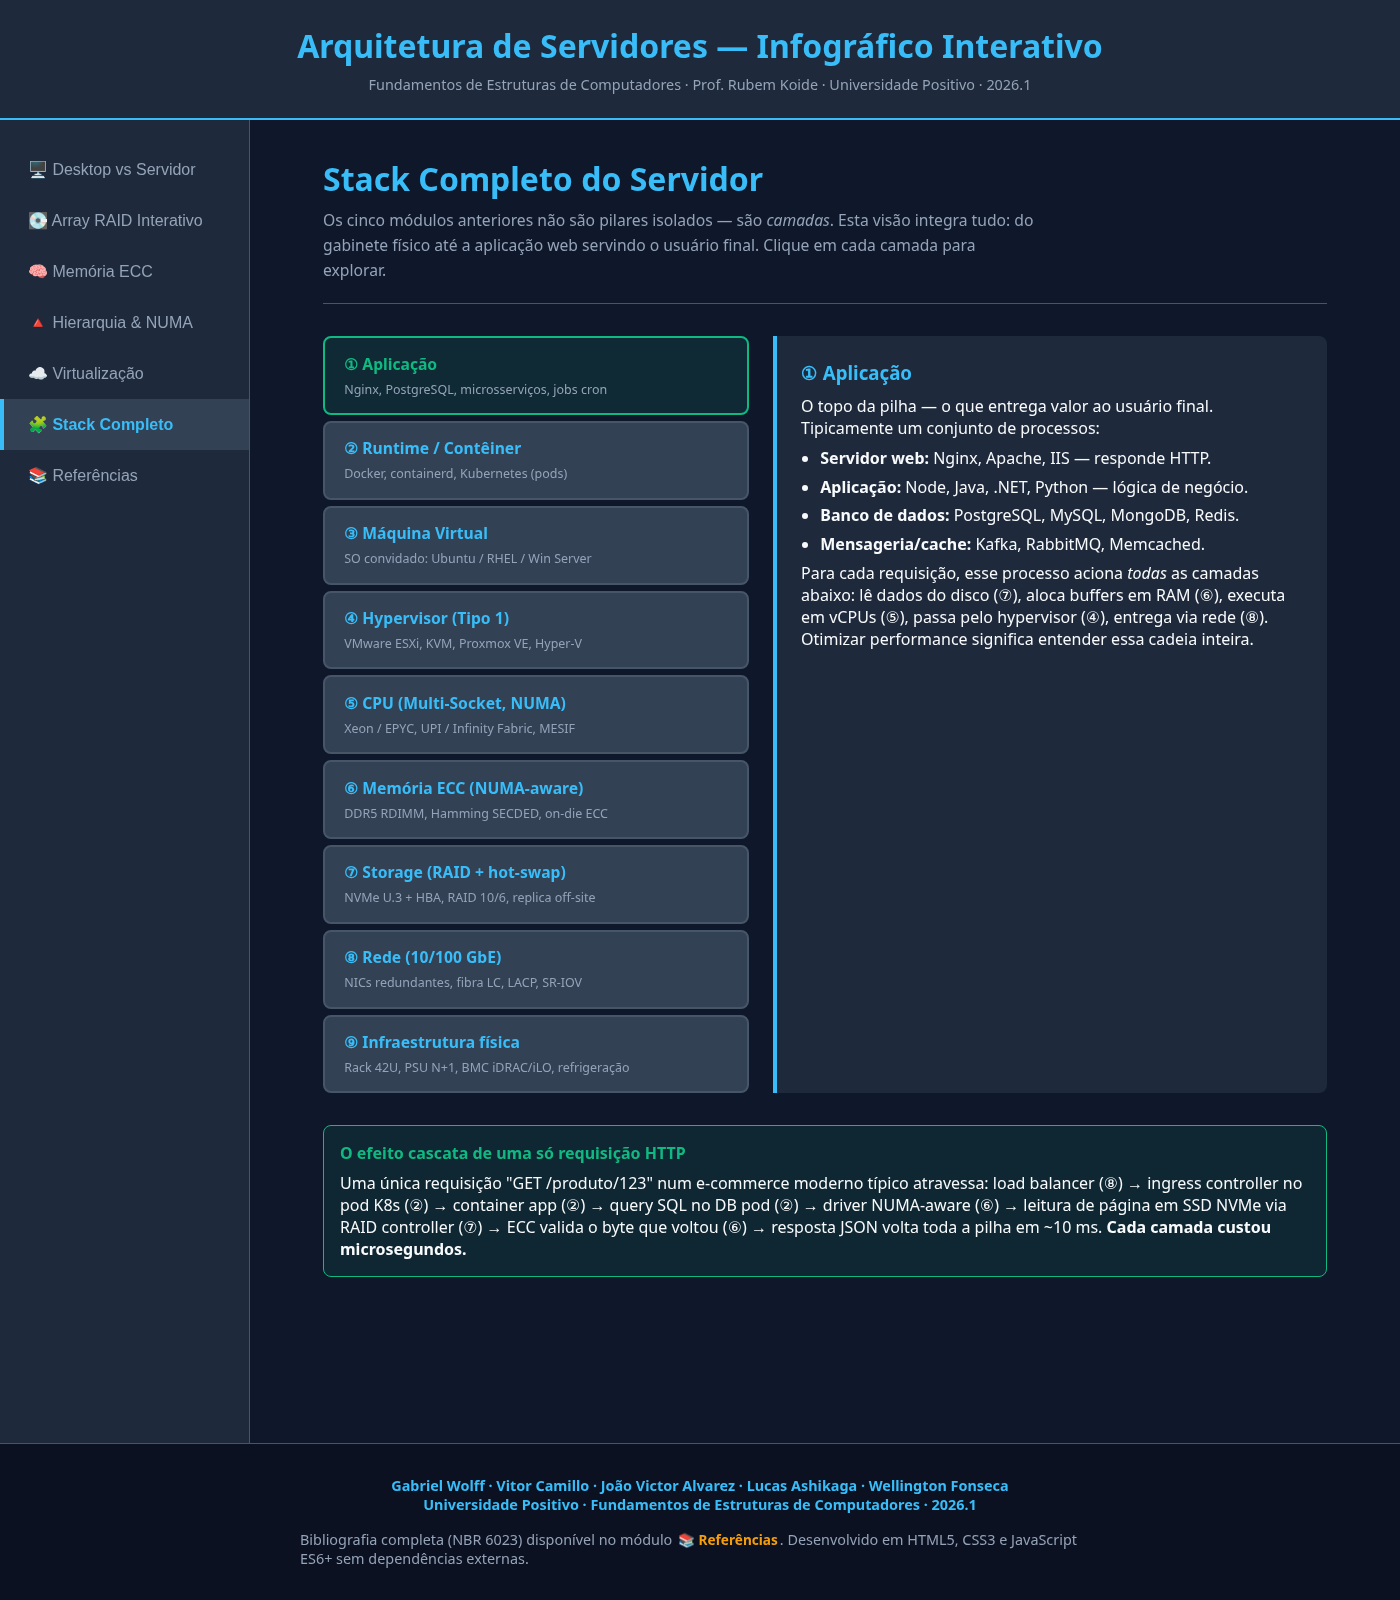
\includegraphics[width=0.95\textwidth]{figuras/mod6.png}
\caption{Módulo 6 --- \emph{Stack} integrado do servidor de produção.}
\label{fig:mod6}
\end{figure}

Este módulo \textbf{não tem sub-abas}: é uma síntese visual integrando
todas as camadas anteriores num único diagrama vertical com 9
camadas clicáveis, do nível físico (PSU, BMC, rack) até a aplicação
no topo (Nginx, PostgreSQL, microsserviços). Ao clicar em cada
camada, o painel à direita exibe seu detalhamento técnico --- com
referências cruzadas aos módulos anteriores.

\subsection{Modelo de dados das camadas}

A informação de cada camada é mantida num objeto JavaScript
\texttt{stackData}, conforme o trecho da Listagem~\ref{lst:stackdata}.

\begin{lstlisting}[language=JavaScript,label=lst:stackdata,caption=Estrutura de dados das camadas do stack]
const stackData = {
    cpu: {
        title: 'CPU (Multi-Socket, NUMA)',
        body:  '<p>Em servidor, 2-8 sockets físicos compartilham ' +
               'a memória via UPI (Intel) ou Infinity Fabric (AMD)' +
               ', com protocolo MESIF/MOESI para coerência.</p>' +
               '<ul><li>Xeon Scalable / EPYC: 16-128 cores/socket</li>' +
               '<li>Hyperthreading: 2 threads lógicos por core físico</li>' +
               '<li>NUMA-aware: scheduler mantém threads próximas à RAM</li>' +
               '</ul>'
    },
    /* ... outras 8 camadas omitidas por brevidade ... */
};
\end{lstlisting}

A função \texttt{showStackDetail(key, el)} troca o painel da direita
para o conteúdo da camada selecionada, mantendo o histórico de
seleção via classe CSS \texttt{.active}.

\section{Módulo de Referências}
\label{sec:mod-ref}

Um sétimo item de navegação --- \textbf{Referências} --- expõe a
lista bibliográfica completa formatada conforme \textsc{abnt}
\textsc{nbr} 6023:2018. Cada citação inline nos módulos é um link
ativo: ao clicar em \texttt{[11]}, por exemplo, o usuário é
transportado para a aba de referências e a entrada $11$ é
destacada em laranja por 2,5 segundos --- comportamento
implementado em \texttt{goToRef(n)}
(Listagem~\ref{lst:gotoref}).

\begin{lstlisting}[language=JavaScript,label=lst:gotoref,caption=Função de navegação para referência citada]
function goToRef(n) {
    showModule('modRef', null);
    setTimeout(() => {
        const target = document.getElementById('ref-' + n);
        if (!target) return;
        target.scrollIntoView({ behavior: 'smooth', block: 'center' });
        target.classList.add('highlight');
        setTimeout(() => target.classList.remove('highlight'), 2500);
    }, 200);
}
\end{lstlisting}

\section{Resultado consolidado}

O artefato final possui:

\begin{itemize}
    \item 6 módulos temáticos + 1 índice de referências;
    \item 21 sub-abas no total (média de 3,5 por módulo);
    \item 17 referências bibliográficas \textsc{abnt} clicáveis;
    \item 11 tabelas técnicas com dados quantitativos;
    \item 8 simulações interativas em JavaScript;
    \item aproximadamente 2\,500 linhas em arquivo HTML único;
    \item \emph{zero} dependências externas, executável \textit{offline}.
\end{itemize}

O salto de profundidade entre as duas iterações pode ser quantificado
de forma simples: a primeira versão do código tinha 1\,060 linhas e
3 referências bibliográficas; a segunda chega a 2\,554 linhas e
17 referências, com adição de todas as fórmulas, tabelas e
simuladores listados acima.
